\documentclass{exammath}
\leadingtext{这里是导语,用\fbox{$\backslash$leadingtext\{文字\}}创建}
\title{这里是标题,用\fbox{$\backslash$title\{文字\}}创建}
\additioninfo{
    \par (i)以上是本包自带的注意事项。若想启用以上事项,只需用\fbox{$\backslash$usebasicinfo}即可。
    \par (ii)以上(及本条、以下)带罗马数字标注的是用户自定义的事项,可以在导语区用$\backslash$additioninfo来创建这样的事项。请注意:必须在该命令中完整地写完所有您需要的东西(包括序号)。当使用\fbox{$\backslash$usebasicinfo}时,自定义的注意事项也会被启用。
    \par (iii)如果不想使用本包自带的事项,可以使用\fbox{$\backslash$useadditioninfoonly}来只启用自定义的事项;或者两个命令皆不使用,取消所有的注意事项。
    \par (iv) 如果需要启用“绝密$\bigstar$启用前”或“机密$\bigstar$启用前”字样,可以使用\fbox{$\backslash$settopsecret}及\fbox{$\backslash$setsecret}实现。
    \par (v)以上(包括本条)中的命令皆在导语区中使用。以下为示例正文。
}
\usebasicinfo

\begin{document}
    \maketitle

    \section{一}{选择题}{本大题共12小题,每小题5分,共60分。在每小题给出的四个选项中,只有一项是符合题目要求的。像这样的大题$\slash$题组,用\fbox{$\backslash$section\{大题序号\}\{大题名称\}\{注解\}}。}
    \simpleproblem 这是一道选择题。对于选择题及填空题,本示例中皆称为“小题”。声明小题时,可以使用\\\fbox{$\backslash$simpleproblem}并后接小题内容。该声明中会自动生成题号,并进行(如本题所示的)悬挂缩进,因此您无须操心于此。但须注意您不能分段。此外,要生成选择题的选项,可以使用\\\fbox{$\backslash$selections\{选项A\}\{选项B\}\{选项C\}\{选项D\}}这样的命令。同样不需关心它的断行问题。
    \selections{选项A}{选项B}{选项C}{选项D}
    \simpleproblem 一个简短的小题示例。
    \selections{选项A}{选项B}{选项C}{选项D}
    \simpleproblem 一个稍长、跨行的小题示例。在工作或学习中遇到不开心的时候,不妨静下来好好想想,自己到底是对是错。生活中不是你对别人好,别人就该对你好,你要明白这个道理,每个人都有自己的原则,有人功利,有人善良,你不可能要求别人什么。
    \selections{选项A}{选项B}{选项C}{选项D}
    \simpleproblem 一个长小题示例。冰灯是流行于中国北方的一种古老的民间艺术形式。因为独特的地域优势,黑龙江可以说是制作冰灯最早的地方。传说在很早以前,每到冬季的夜晚,在松嫩平原上,人们总会看到三五成群的农夫和渔民在悠然自得地喂马和捕鱼,他们所使用的照明工具就是用冰做成的灯笼。这便是最早的冰灯。当时制作冰灯的工艺也很简单,把水放进木桶里冻成冰坨,凿出空心,放个油灯在里面,用以照明,冰罩挡住了凛冽的寒风,黑夜里便有了不灭的灯盏,冰灯成了人们生活中不可缺少的帮手。后来,每逢新春佳节和上元之夜,人们又把它加以装饰,而成为供人观赏的独特的艺术表现形式。清代《黑龙江外纪》里对此有过详细的记载:“上元,城中张灯五夜,村落妇女来观剧者,车声彻夜不绝。有镂五六尺冰为寿星灯者,中燃双炬,望之如水晶人。”其时,冰灯在南方一些地方也相继出现过。乾隆、嘉庆年间,四川诗人张问陶曾写过一首专门描写冰灯的诗,题名就叫《冰灯》,诗云:“黑夜有炎凉,冰灯吐焰长。照来消热念,凿处漏寒光。影湿星沉水,神清月里霜。三冬足文史,底用探萤囊。”南京诗人金德荣在被谪戍新疆巴里坤时,在其古风长诗《巴里坤冰灯歌》中也咏叹道:“雪山高与天山接,上有万古不化雪。朔风一夜结作冰,裁雪妙手搏为冰。以矾入冰冰不化,以烛照冰光四射。五里之内尽通明,半月能教天不夜。元夕月轮照碧空,大千人入水晶宫。”
    \selections{选项A}{选项B}{选项C}{选项D}
    \simpleproblem 一个长选项示例。\textbf{请尽量不要使用过长的选项。}
    \selections{冰灯是流行于中国北方的一种古老的民间艺术形式}{因为独特的地域优势,黑龙江可以说是制作冰灯最早的地方。}{传说在很早以前,每到冬季的夜晚}{在松嫩平原上}
    \begin{center}
        \begin{minipage}[c]{.65\textwidth}
            \par
            \setindent{2.7ex}
            \simpleproblem 一个右侧图片示例。由于该包可能不兼容wrapfig,picinpar等插图用宏包,同时为了便于手动操纵,请手动用\fbox{minipage}环境进行操控。目前版本下在用该法插侧图时会出现缩进问题,因此请暂时自行修正。建议:对两minipage居中排列,文字区用0.65倍空间,图片区用0.25倍空间,文字区缩进改为2.7ex。暂时修改缩进,可以在声明前用提供的\fbox{$\backslash$setindent\{新缩进\}}命令实现。
        \end{minipage}
        \begin{minipage}[c]{.25\textwidth}
            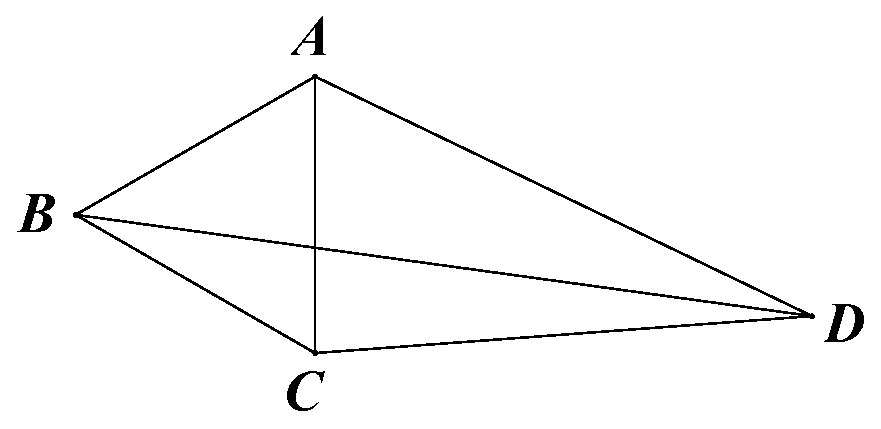
\includegraphics[width=\textwidth]{21-1.eps}
        \end{minipage}
    \end{center}
    \selections{选项A}{选项B}{选项C}{选项D}
    
    \simpleproblem 一个未完成的小题示例。
    \selections{选项A}{选项B}{选项C}{选项D}
    \simpleproblem 一个未完成的小题示例。
    \selections{选项A}{选项B}{选项C}{选项D}
    \simpleproblem 一个未完成的小题示例。
    \selections{选项A}{选项B}{选项C}{选项D}
    \simpleproblem 一个未完成的小题示例。
    \selections{选项A}{选项B}{选项C}{选项D}
    \simpleproblem 一个未完成的小题示例。
    \selections{选项A}{选项B}{选项C}{选项D}
    \simpleproblem 一个未完成的小题示例。
    \selections{选项A}{选项B}{选项C}{选项D}
    

\end{document}